\newpage

\section{Analysis}

\subsection{Users}

The \code{users.csv} file contains records of 19,925,838 (around 20 million) users.

\subsubsection{Exponential Growth}

After launching in 2007, GitHub has been growing exponentially, which is made evident from Figure 1.

\begin{figure}[htb]
\centering
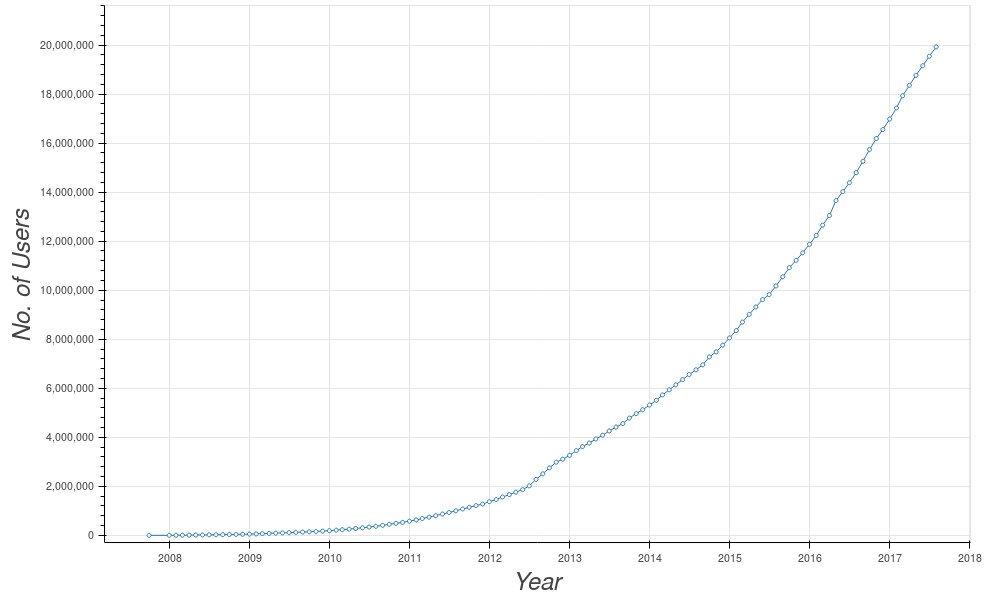
\includegraphics[scale=0.35]{users-exponential-growth}
\caption{User growth rate}
\end{figure}


% \newpage
\subsubsection{New users per Year-Month}

Figure 2 shows that May, 2016 was the month in which most new users were added to the site.

\begin{figure}[htb]
\centering
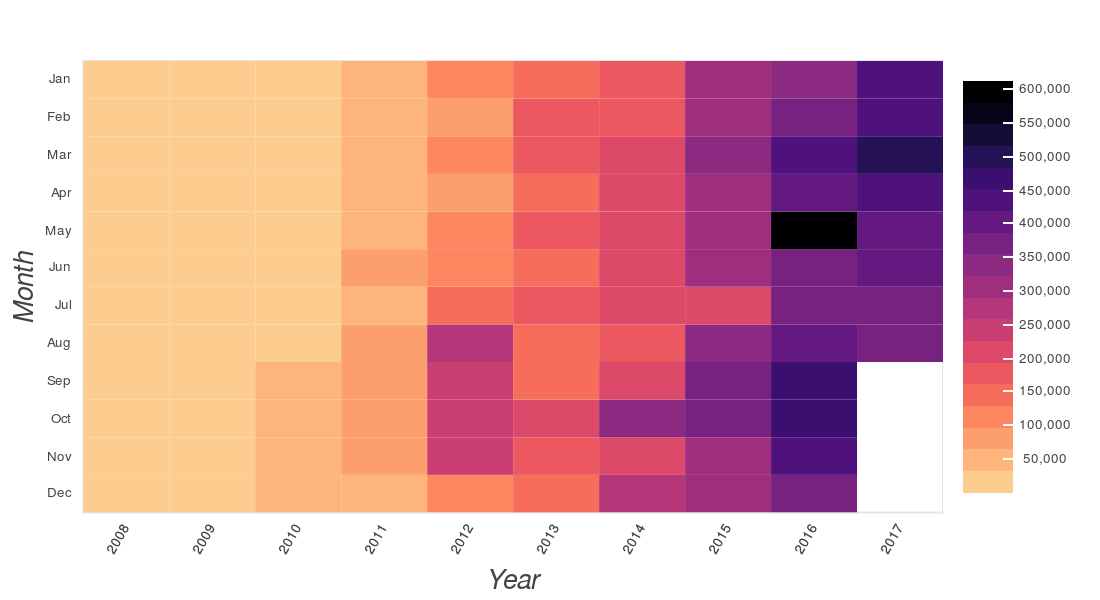
\includegraphics[scale=0.35]{user-year-month}
\caption{New users added per Year-Month}
\end{figure}

\subsubsection{User distribution across countries}

GitHub allows users to enter their location field in a free form text field.
Since this user entered data is not validated by GitHub, it can contain anything and does not have to be a valid location.
GHTorrent service uses mapping APIs like Bing \& Open Street Maps to convert the text data into known locations. \\

Since not everyone enters their location and or they don't enter it in a valid format, only 7.8\% (1,566,019)
 users have location data that can be used. \\

Figure 3 shows that majority of such users are from USA, followed closely by India and China.

% TODO: Pie Chart for countries

\begin{figure}[htb]
\centering
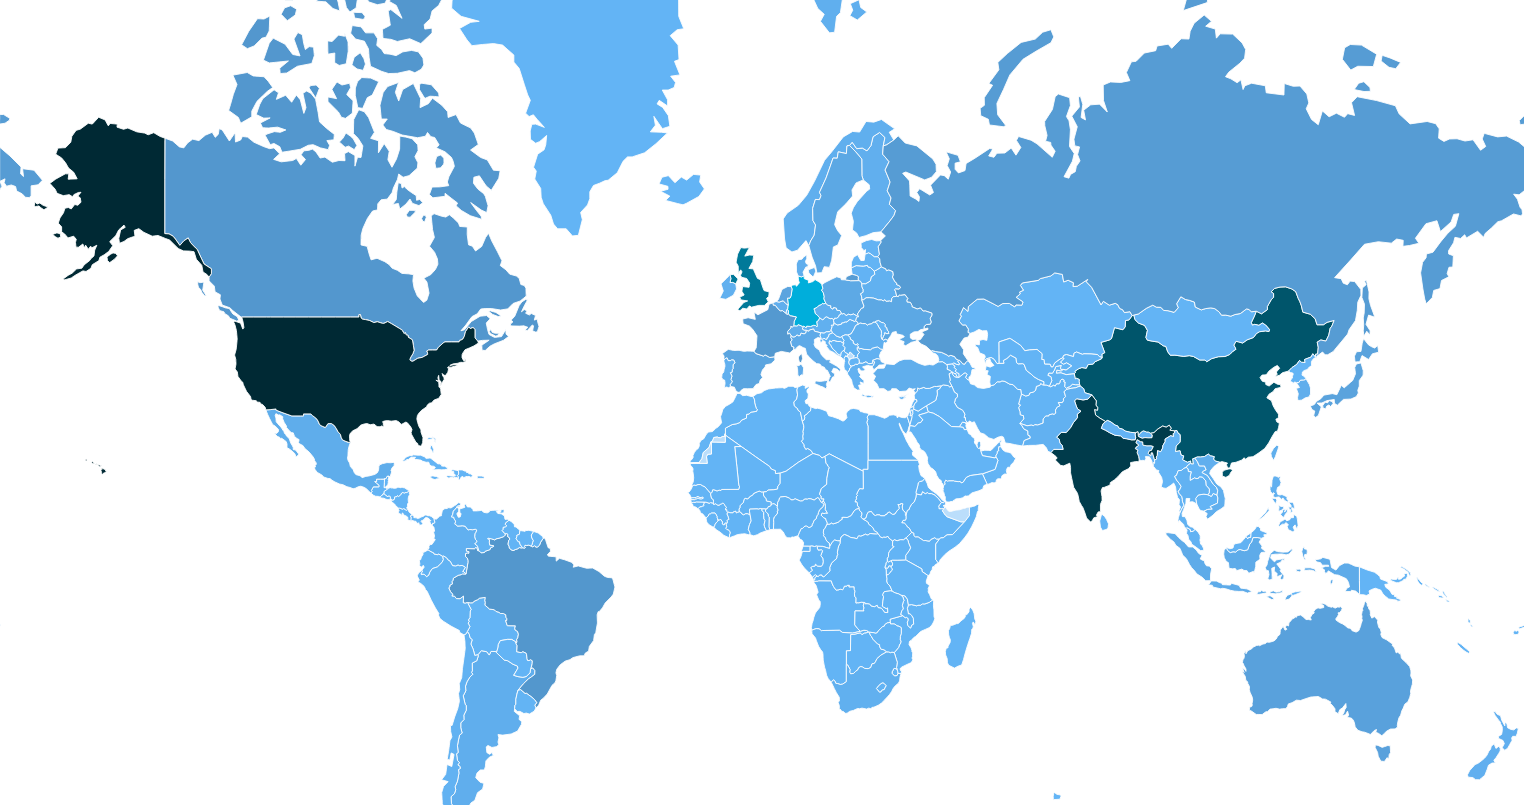
\includegraphics[scale=0.23]{users-country}
\caption{User distribution across countries}
\end{figure}

\subsubsection{User distribution across India}

Of the 1.5 million users with mappable location data, only 102,505 are from India.
Their state-wise distribution is given in Figure 4. \\

As can be seen, most GitHub users are from Karnataka and Maharashtra as they are home to
IT Hubs like Hyderabad, Bengalore, Pune etc.

\begin{figure}[htb]
\centering
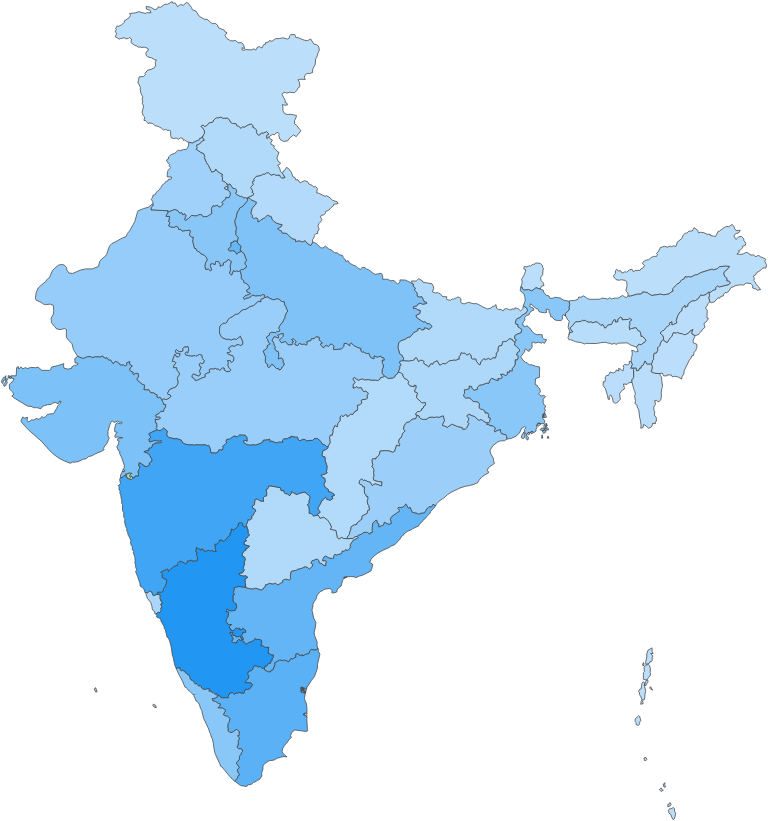
\includegraphics[scale=0.20]{users-india-state}
\caption{User distribution across India}
\end{figure}

\subsection{Organizations}

\subsubsection{Top Organizations}

On GitHub, users can enter the company the work for in a free form text field.
We use that data to find out which organizations have most number of users.
Considering only the number of employees of organizations,
Microsoft has most number of employees i.e 8148, while IBM only has 2842. (Figure 5) \\

Another way of finding popular organizations is to see how popular the work done by
their users is. This is done by counting their followers and the stars on their repositories.
we find that Facebook \& Google are at top, perhaps due to a large number of popular projects.

\begin{figure}[htb]
\centering
\centerline{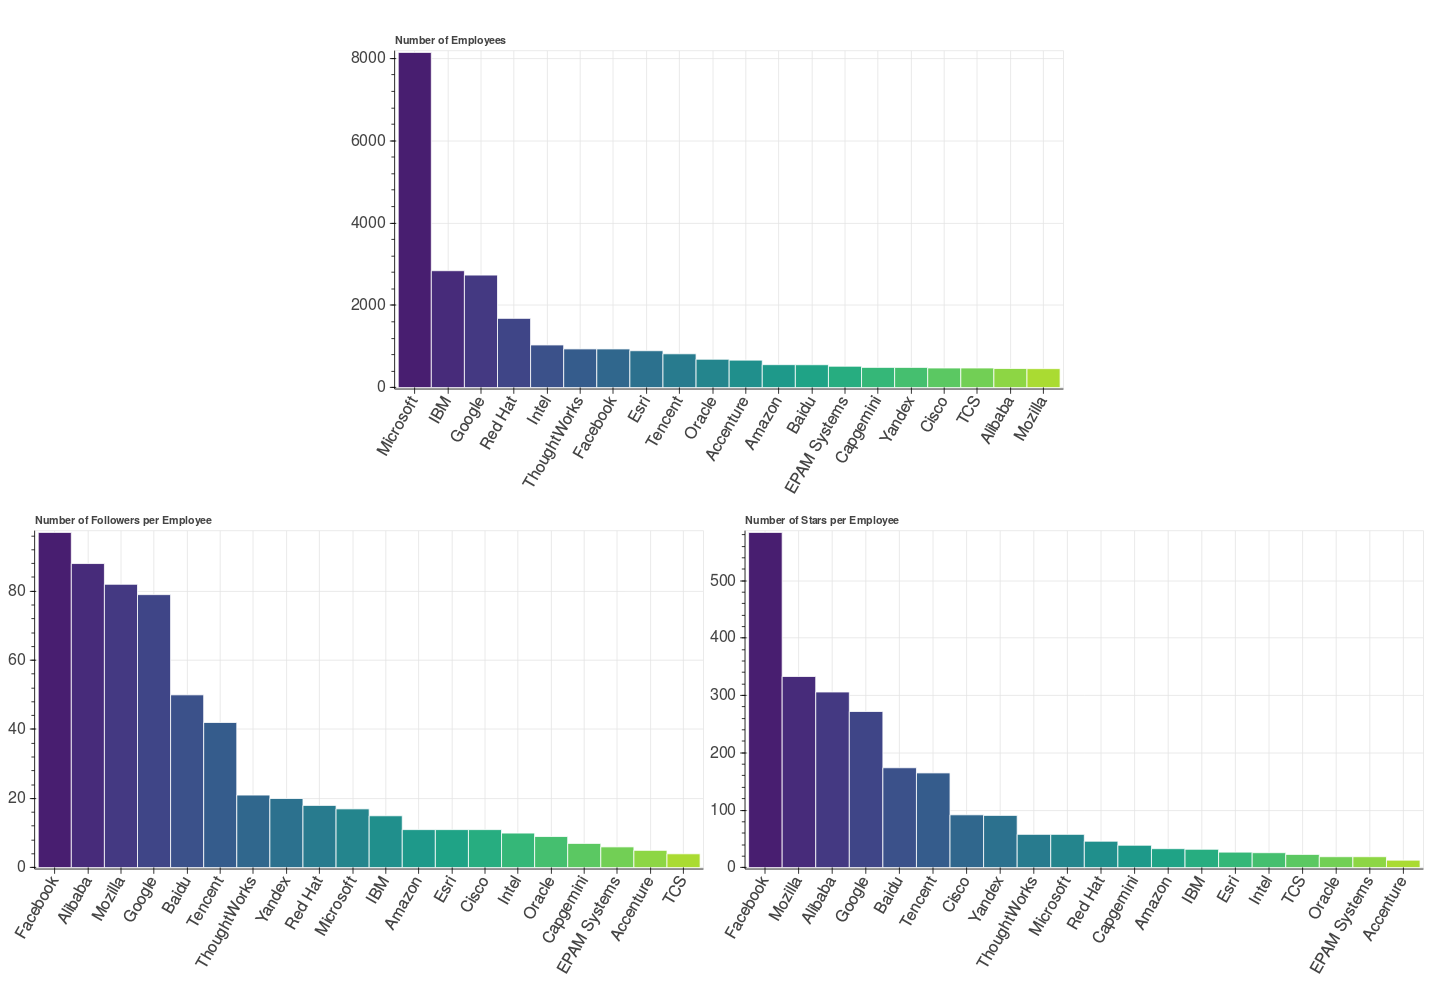
\includegraphics[scale=0.50]{org-employee-full}}
\caption{Organisations with most employees (on GitHub)}
\end{figure}

\newpage

\subsubsection{Top Organizations in India}

Extending similar analysis onto organizations whose employees are located in India, we find that
TCS has the most employees.

\begin{figure}[htb]
\centering
\centerline{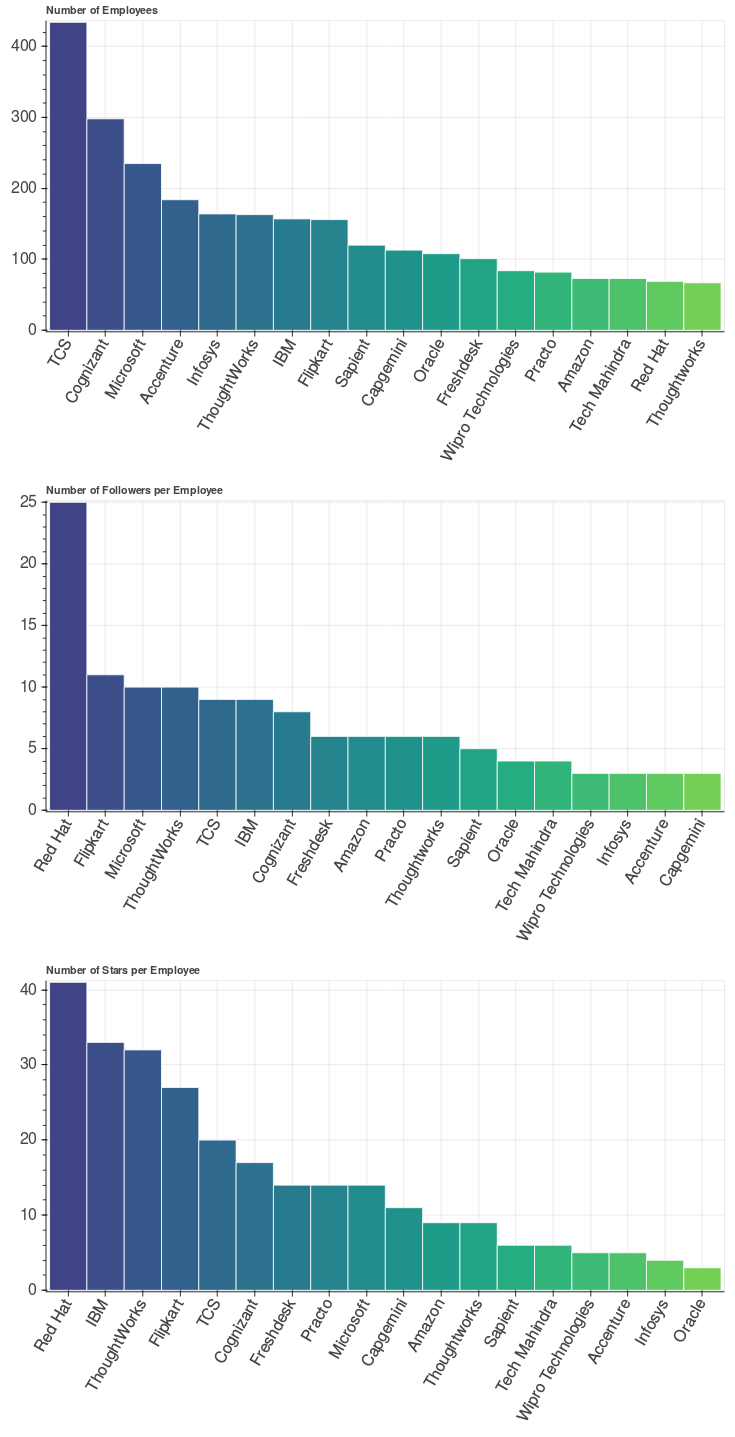
\includegraphics[scale=0.50]{org-employee-full-indian}}
\caption{Organisations with most Indian employees}
\end{figure}

\newpage
\subsubsection{Users at IITs}

\begin{figure}[htb]
\centering
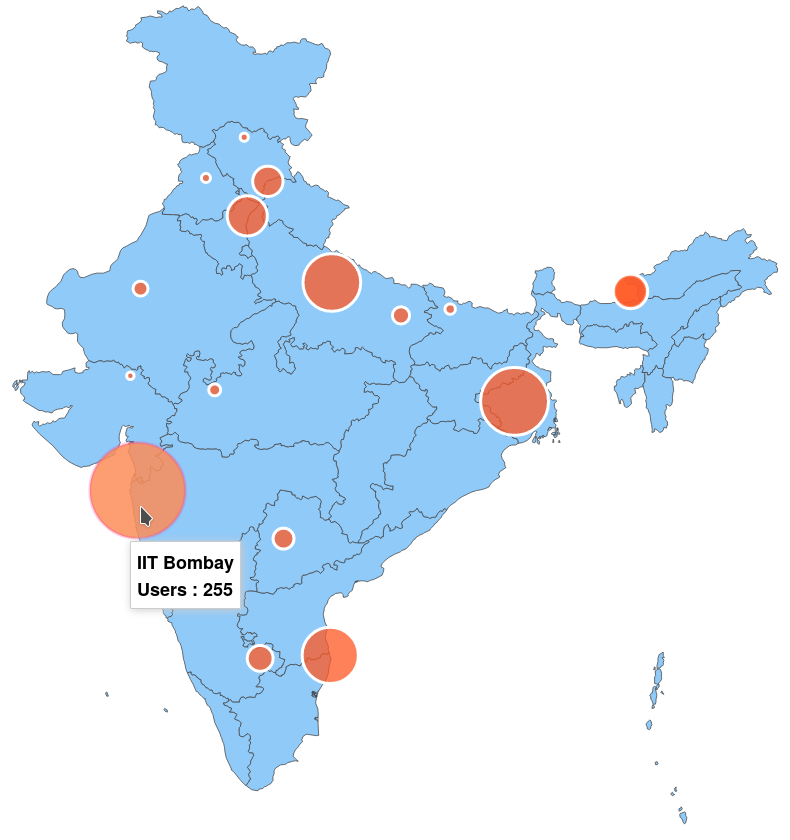
\includegraphics[scale=0.55]{indian-institutes}
\caption{Number of users from various IITs}
\end{figure}

\newpage
\subsection{Activities}

GitHub has a multiple forms of activities that a user can perform on the site - Commits, Issues, Pull Requests.
It should be noted that GitHub treats pull request as a special form of Issues. \\

\code{commits.csv} contains information of 745,356,807 commits made during 2007 and 2017.

\subsubsection{Commit patterns of users}

To determine when a user works, we plot a punchcard created using the timestamps of the commits.
This is created by considering the users's local timezone (since the GHTorrent data stores it in UTC.) \\

Comparing Figure 5 \& 6, it is clear that both these users have very different work schedules.

\begin{figure}[htb]
\centering
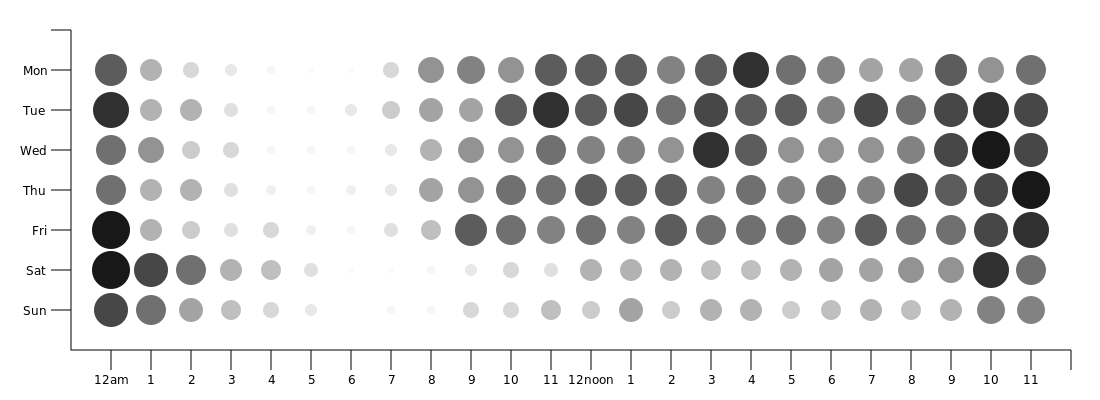
\includegraphics[scale=0.28]{commits-punchcard-JakeWharton}
\caption{Commit punchcard of user "JakeWharton"}
\end{figure}

\begin{figure}[htb]
\centering
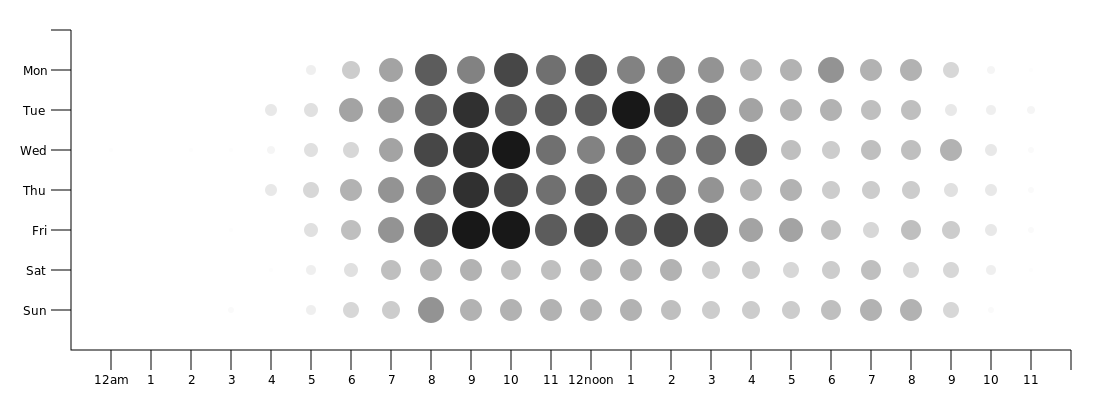
\includegraphics[scale=0.28]{commits-punchcard-mbostock}
\caption{Commit punchcard of user "mbostock"}
\end{figure}

This can also be extended to entire countries to see when people of a country commit to GitHub.

\begin{figure}[htb]
\centering
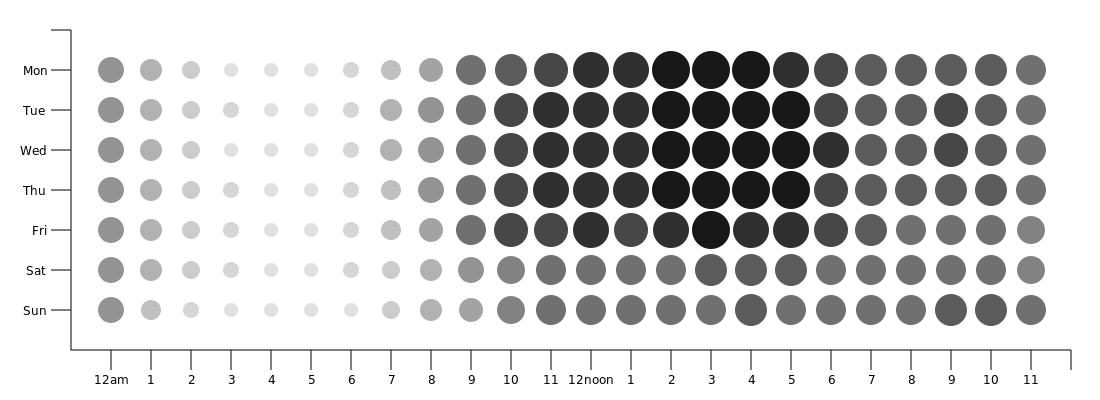
\includegraphics[scale=0.28]{commits-punchcard-indian}
\caption{Commit punchcard of all Indian users}
\end{figure}

\newpage
\subsubsection{Community participation in projects}

We defined community participation as the percentage of commits in a repository that were made
by someone other than the owner. By analysing the commits data we found that most of the projects
on GitHub have 0 participation from others, which means they are done by a single person.

\begin{figure}[htb]
\centering
\centerline{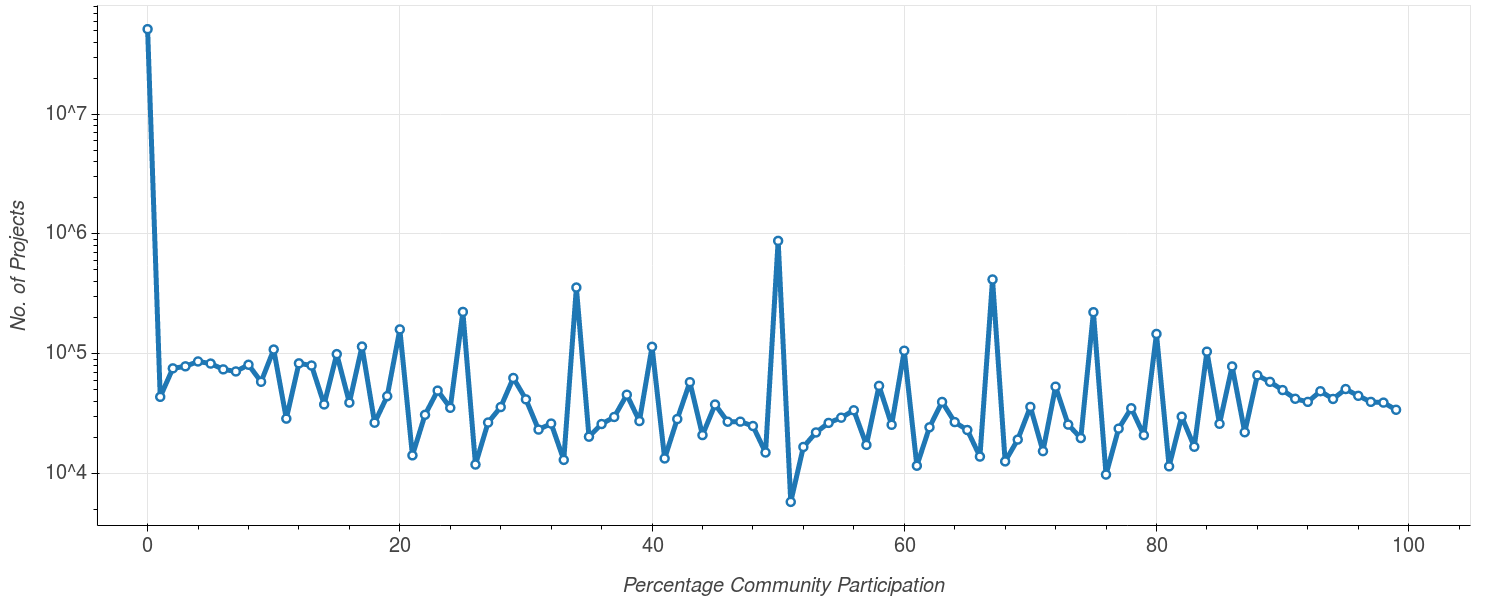
\includegraphics[scale=0.35]{community-participation}}
\caption{Community participation in projects}
\end{figure}

\subsubsection{Programming Language Popularity}

The \code{project\_languages.csv} file contains information on usage of Programming Languages.
In Figure 12, we plot the usage of top 10 languages (by their code size in GB). \\

The data shows that by absolute code size, C was the most used language in 2015 \& 2016, while
Javascript was the most used in 2017.

\begin{figure}[htb]
\centering
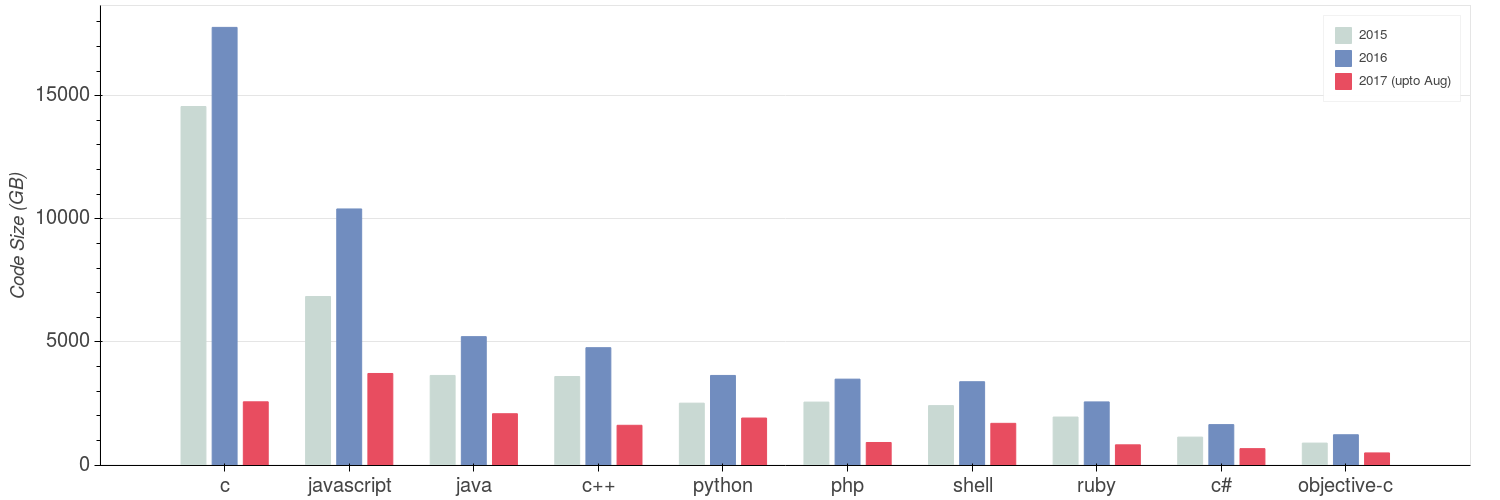
\includegraphics[scale=0.30]{top-language-year}
\caption{Top 10 programming languages}
\end{figure}
